\documentclass[journal]{IEEEtran}

\usepackage{cite}
% http://www.ctan.org/tex-archive/macros/latex/contrib/cite/
\usepackage[pdftex]{graphicx}
\graphicspath{{./img/}}
\DeclareGraphicsExtensions{.pdf,.jpeg,.png}
\usepackage{algorithmicx}
% http://www.ctan.org/tex-archive/macros/latex/contrib/algorithmicx/
\usepackage{array}
% http://www.ctan.org/tex-archive/macros/latex/required/tools/
\usepackage{mdwtab}
% http://www.ctan.org/tex-archive/macros/latex/contrib/mdwtools/
\usepackage{eqparbox}
% http://www.ctan.org/tex-archive/macros/latex/contrib/eqparbox/
\usepackage[caption=false,font=footnotesize]{subfig}
% http://www.ctan.org/tex-archive/macros/latex/contrib/subfig/
\usepackage{fixltx2e}
% http://www.ctan.org/tex-archive/macros/latex/base/
\usepackage{stfloats}
% http://www.ctan.org/tex-archive/macros/latex/contrib/sttools/
\usepackage{url}
% http://www.ctan.org/tex-archive/macros/latex/contrib/misc/

% correct bad hyphenation here
\hyphenation{op-tical net-works semi-conduc-tor}


\begin{document}

\title{WWW-Graphics-Module for Mixed-Reality-System}

\author{Hannes~Eilers,~\textit{Master-student,~Chairman~student~group~NorthernStars,~FH-Kiel,}
        Eike~Petersen,~\textit{Master-student,~FH-Kiel}}

% The paper headers
\markboth{Advanced JavaScript project paper, January~2014}%
{Shell \MakeLowercase{\textit{et al.}}: WWW-Graphics-Module for Mixed-Reality-System}

\maketitle

\begin{abstract}
	Warum? Was? Wie? (Max 200 W)
\end{abstract}
\begin{IEEEkeywords}
mixed-reality, javascript, server, client, paper.
\end{IEEEkeywords}

\section{Introduction}

\IEEEPARstart{H}{ier} steht was ueber Northernstars, MixedReality und so AJS Projektbedingungen usw steht was ueber Northernstars, MixedReality und so AJS Projektbedingungen uswsteht was ueber Northernstars, MixedReality und so AJS Projektbedingungen uswsteht was ueber Northernstars, MixedReality und so AJS Projektbedingungen uswsteht was ueber Northernstars, MixedReality und so AJS Projektbedingungen uswsteht was ueber Northernstars, MixedReality und so AJS Projektbedingungen uswsteht was ueber Northernstars, MixedReality und so AJS Projektbedingungen uswsteht was ueber Northernstars, MixedReality und so AJS Projektbedingungen uswsteht was ueber Northernstars, MixedReality und so AJS Projektbedingungen uswsteht was ueber Northernstars, MixedReality und so AJS Projektbedingungen uswsteht was ueber Northernstars, MixedReality und so AJS Projektbedingungen uswsteht was ueber Northernstars, MixedReality und so AJS Projektbedingungen uswsteht was ueber Northernstars, MixedReality und so AJS Projektbedingungen uswsteht was ueber Northernstars, MixedReality und so AJS Projektbedingungen uswsteht was ueber Northernstars, MixedReality und so AJS Projektbedingungen uswsteht was ueber Northernstars, MixedReality und so AJS Projektbedingungen uswsteht was ueber Northernstars, MixedReality und so AJS Projektbedingungen uswsteht was ueber Northernstars, MixedReality und so AJS Projektbedingungen uswsteht was ueber Northernstars, MixedReality und so AJS Projektbedingungen uswsteht was ueber Northernstars, MixedReality und so AJS Projektbedingungen uswsteht was ueber Northernstars, MixedReality und so AJS Projektbedingungen uswsteht was ueber Northernstars, MixedReality und so AJS 

\subsection{Project definition (Was machen wir?)}
The projects goal is to bring the local mixed-reality-games to an audience everywhere in the world (Figure~\ref{fig:proj_goal}). All that is needed is a device with a HTML-5 compliant Browser and an internet-connection with a bit-rate of at least 10-kbit/s downstream.
\begin{figure}[!t]
    \centering
    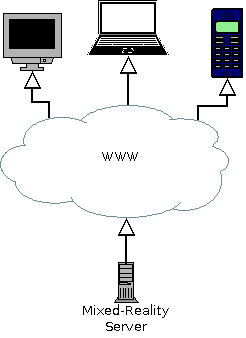
\includegraphics[width=0.3\textwidth]{project-target.png}
    \caption{Project goal: Bringing MR to you!}
    \label{fig:proj_goal}
\end{figure}
The primarily targeted devices are pcs, tablets and smart-phones but not limited to those. \\
The games should be streamed in real-time from the mixed-reality game-server over a web-server to in-browser RICH-clients, where they will be displayed in the same fashion as the local mixed-reality-game graphics.
\subsection{Design (Wie sieht es aus?)}


\subsection{Implementation(Wie ist es aufgebaut?)}


\section{Conclusion}
Ergebnis Auswertung und weitere Aussichten

\appendices
\section{Proof of the First Zonklar Equation}
Appendix one text goes here.

\section*{Acknowledgment}

The authors would like to thank...

\begin{thebibliography}{1}

\bibitem{IEEEhowto:kopka}
H.~Kopka and P.~W. Daly, \emph{A Guide to \LaTeX}, 3rd~ed.\hskip 1em plus
  0.5em minus 0.4em\relax Harlow, England: Addison-Wesley, 1999.

\end{thebibliography}

\end{document}


